%%%%%%%%%%%%%%%%%%%%%%%%%%%%%%%%%%%%%%%%%%%%%%%%%%%%%%%%%%%%
% Paul McKee
% Rensselaer Polytechnic Institute
% 1/31/18
% Master's Thesis
% with Dr. Kurt Anderson
% LaTeX Template: Project Titlepage Modified (v 0.1) by rcx
%%%%%%%%%%%%%%%%%%%%%%%%%%%%%%%%%%%%%%%%%%%%%%%%%%%%%%%%%%%%

\documentclass[12pt]{article}

%\usepackage[demo]{graphicx}
\usepackage{caption}
\usepackage{subcaption}

\usepackage{blindtext}
\usepackage[utf8]{inputenc}

\usepackage{graphicx, wrapfig, subcaption, setspace, booktabs}
\usepackage{sectsty}
\usepackage{url, lipsum}
\usepackage{makecell}
\usepackage{amsmath}
\usepackage{setspace}
\usepackage{amsmath}
\usepackage{color} %red, green, blue, yellow, cyan, magenta, black, white
\definecolor{mygreen}{RGB}{28,172,0} % color values Red, Green, Blue
\definecolor{mylilas}{RGB}{170,55,241}

\usepackage[table,xcdraw]{xcolor}


\usepackage[margin=.75in]{geometry} 
\usepackage{amsmath,amsthm,amssymb}
\usepackage{color}
\usepackage{fancyhdr}
\usepackage{lastpage}
\usepackage{graphicx}

\usepackage{cite}%AddedbyChris
\usepackage{graphicx}%AddedbyChris
\usepackage{array}%Added by Chris
\usepackage{caption}
\usepackage{amsmath}%Added by Chri
\pagestyle{fancy}
\fancyhf{}
%\fancyhead[L]{Independant Study}
%\fancyhead[C]{\rightmark}
\fancyhead[C]{}

\fancyhead[L]{\nouppercase{\leftmark}}
\fancyhead[R]{Philip Hoddinott}

\rfoot{Page \thepage \hspace{1pt} of \pageref{LastPage}}

\newcommand{\N}{\mathbb{N}}
\newcommand{\Z}{\mathbb{Z}}
\newcommand{\norm}[1]{\left\lVert#1\right\rVert}

\newenvironment{theorem}[2][Theorem]{\begin{trivlist}
		\item[\hskip \labelsep {\bfseries #1}\hskip \labelsep {\bfseries #2.}]}{\end{trivlist}}
\newenvironment{lemma}[2][Lemma]{\begin{trivlist}
		\item[\hskip \labelsep {\bfseries #1}\hskip \labelsep {\bfseries #2.}]}{\end{trivlist}}
\newenvironment{exercise}[2][Exercise]{\begin{trivlist}
		\item[\hskip \labelsep {\bfseries #1}\hskip \labelsep {\bfseries #2.}]}{\end{trivlist}}
\newenvironment{problem}[2][Problem]{\begin{trivlist}
		\item[\hskip \labelsep {\bfseries #1}\hskip \labelsep {\bfseries #2.}]}{\end{trivlist}}
\newenvironment{question}[2][Question]{\begin{trivlist}
		\item[\hskip \labelsep {\bfseries #1}\hskip \labelsep {\bfseries #2.}]}{\end{trivlist}}
\newenvironment{corollary}[2][Corollary]{\begin{trivlist}
		\item[\hskip \labelsep {\bfseries #1}\hskip \labelsep {\bfseries #2.}]}{\end{trivlist}}

\newenvironment{solution}{\begin{proof}[Solution]}{\end{proof}}
\usepackage{multicol}
\newcommand{\mysize}{0.5}
\usepackage{subcaption}
\usepackage{float}
\usepackage{listings}
\usepackage{color} 
\newcolumntype{L}{>{\centering\arraybackslash}m{3cm}}
\usepackage{setspace}
\usepackage[framed,numbered,autolinebreaks,useliterate]{mcode}

\newlength\longest

% %---------------------------------------------------------------
% % HEADER & FOOTER
% %---------------------------------------------------------------

%\fancyhf{}
%\pagestyle{fancy}
%\renewcommand{\headrulewidth}{0pt}
%\setlength\headheight{0pt}
%\fancyhead[L]{ Paul McKee }
%\fancyhead[R]{Rensselaer Polytechnic Institute}
%\cfoot{ \thepage\ } 


%--------------------------------------------------------------
% TITLE PAGE
%--------------------------------------------------------------
\iffalse
\begin{titlepage}
	\title{ 
		\LARGE \textbf{\uppercase{Put Title Here}} \\
		\vspace{0.25cm}
		\LARGE \textbf{Philip Hoddinott}
	}
	\author{\small{Submitted in Partial Fulfillment of the Requirements} \\ \small{for the Degree of} \\
		\uppercase{Master of Science} \\ \\
		Approved by:
		\\ Kurt Anderson, Chair \\ John Christian \\ Matthew Oehlschlaeger \\ \\ %% from paul's template
		\includegraphics[width=2.5cm]{rensselaer_seal.png} \\
		\small{\textit{Department of Mechanical, Aerospace, and Nuclear Engineering}} \\
		\small{Rensselaer Polytechnic Institute} \\ 
		\small{Troy, New York} \\
		\small{November 2018}
	}
\end{titlepage}
\fi

\begin{document}
		\title{Deep Neural Network}
	\author{Philip Hoddinott}
	
	\maketitle
	%\pagenumbering{roman}
	%\thispagestyle{empty}
	%\clearpage


	
	%\newpage


	%\thispagestyle{fancy}
	
	%\addcontentsline{toc}{section}{\uppercase{Table of Contents}}
	%\listoftables
	%\addcontentsline{toc}{section}{\uppercase{List of Tables}}
	%\listoffigures
	%\addcontentsline{toc}{section}{\uppercase{List of Figures}}
	% -----------------------------
	
	% ------------------------------------------------------------
	% Acknowledgement
	% ------------------------------------------------------------



	
	% ------------------------------------------------------------
	% Abstract 
	% ------------------------------------------------------------
	
	\newpage
	\section*{Abstract}
	\textcolor{red}{Remove pasive voice, will, chec out rubirc }
	The purpose of this report is to develop a neural net that can identify handwritten digets in the MNIST database at near human levels of accuracy. The neural net will be developed without the assistance of libraries such as Python's tensor flow or MATLAB's Deep Learning. 
	
	solve the MNIST  on the mnist database
	. \par 
	The author would like to express his gratitude to Professor Hicken
	
	
	 for his suggestion of this project and his assistance with the methods of orbital determination through out the semester.\par 
	
		\newpage
%\setcounter{page}{1}
\tableofcontents
\listoffigures
\doublespacing
	%\textcolor{red}{ Do More}
	% ------------------------------------------------------------
	% Introduction
	% ------------------------------------------------------------
	\newpage
	 % this should start the normal numberinbg

	\section{Introduction}
	Have it solve the MNIST with a simple simple thing
	then try diffrent layers and stuff
	
	Go over tan h vs sigmoid\
	Explain batch testing
	

	\subsection{The MNIST database}
	The Modified National Institute of Standards and Technology database or MNIST database\cite{mnistDATABASE} is a database of handwritten numbers used to train image processing systems. It contains 60,000 training images and 10,000 testing images. 
	
	A number of attempts have been made to get the lowest possible error rate on this dataset. As of August 2018 the  the lowest achieved so far is a error rate of 0.21\% or an accuracy of 99.79\%. For comparison human can accurately recognize digits at a rate of 98.5\%\cite{humanPerf}.
	
	The database is comprised of images that are made up of a grid of 28x28 pixels. Some of these are seen in figure \ref{fig:mathworksmnistneuralnetfinal}. 
	
	\begin{figure}[H]
		\centering
		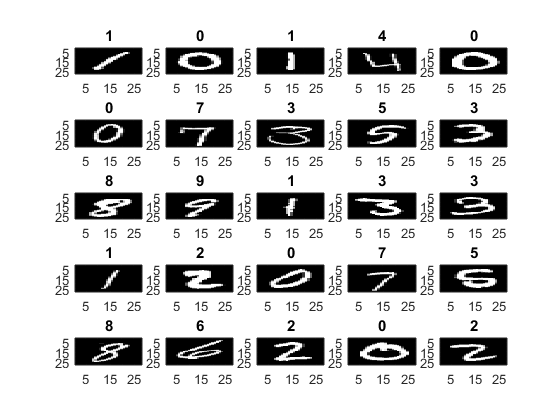
\includegraphics[width=0.7\linewidth]{mathworks_mnist_neuralnetFinal}
		\caption{Sample numbers from MNIST \cite{matlabNNBeg}.}
		\label{fig:mathworksmnistneuralnetfinal}
	\end{figure}
	
	\subsection{Artificial neural network}
	An artificial neural network (referred tp as a neural network in this paper) is a computation system that mimics the biological neural netwroks found in animal brains. A nerual network is not an explict
	A 
	Neural networks may be trained for tasks, such as the number recognition in this report. 
	
	\begin{figure}
		\centering
		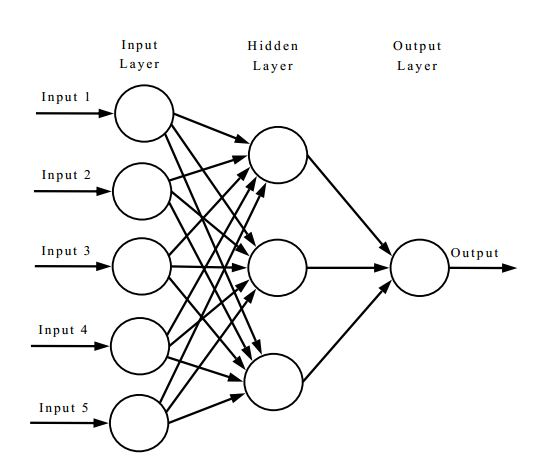
\includegraphics[width=0.6\linewidth]{nnDiagram}
		\caption{Visualization of a neural network \cite{nnDiagramStack}. }
		\label{fig:nndiagram}
	\end{figure}
	
	
	\subsection{Neural Network Walkthrough}
	
	Forward and backward propogation are visulized in figure \ref{fig:forwardbackwardprop}
	\begin{figure}
		\centering
		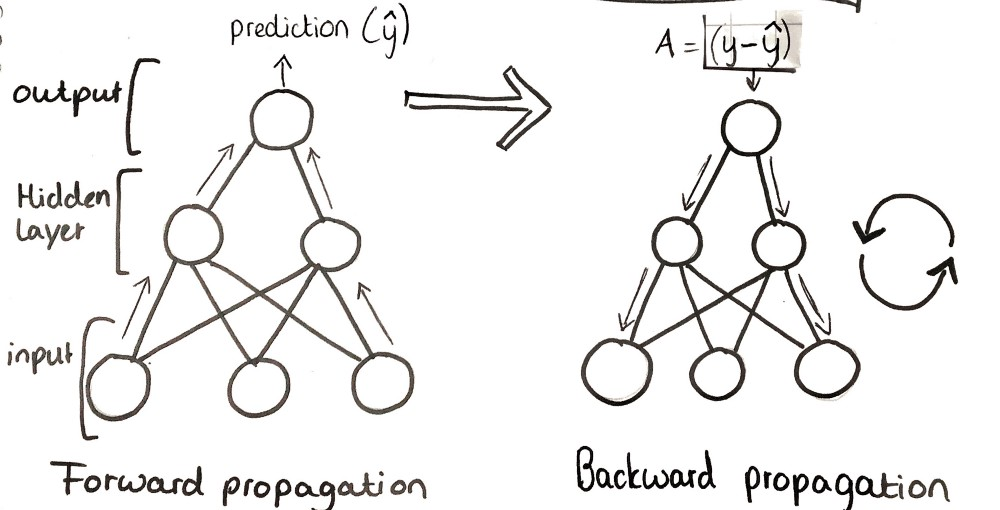
\includegraphics[width=0.7\linewidth]{forwardBackwardProp}
		\caption{A visulization of forward and backward propogation \cite{nnBlog}.}
		\label{fig:forwardbackwardprop}
	\end{figure}

	The four steps
	\begin{enumerate}\singlespacing
		\item Initialize weights and biases. 
		\item Forward propagation
		\item compute loss
		\item back prop
	\end{enumerate}\doublespacing
	\subsubsection{Parameter Initialization}
	The first step in training a neural net is to initialized the bias vectors and weight  matrices. They are initialized with random numbers between 0 and 1, then multiplied by a small scalar around the order of $10^{-2}$ so that the units are not on the region where the derivative of the activation function are close to zero. The initial parameters should be different values (to keep the gradients from being the same).
	
	There are various forms of initialization such as Xavier initialization or He-et-al Initialization, but a discussion on methods of initialization outside the scope of this paper. In this paper we will stick with random parameter initialization. 
	
	

	\subsubsection{Forward Propagation}
	The next step is the forward propagation. The network takes the inputs from a previous layer, computes their transformation, and applies an activation function. Mathematically this is represented by equation \ref{eqn:forProp}. 
	\begin{equation}
	\begin{aligned}
	z_i = A_{i-1}* W_{i}+b\\
	A_i=\phi(z_i)
	\end{aligned}
	\label{eqn:forProp}
	\end{equation}
	Where z is the input vector, A is the layer, W is the weights going into the layer, b the bias, and $\phi$ the activation function. This process then repeats for the next layer until it reaches the end of the neural net.
	
	\subsubsection{Cost}
	The cost or the loss

	\subsubsection{Backward propagation}
	
	After going forward through the neural net in the forward propagation step, the next step is backwards propagation. Backwards propagation is the updating of the weight parameters via the derivative of the error function with respect to the weights of the neural net. For the output layer this is seen in equation \ref{eqn:outputBack} and equation \ref{eqn:allOtherBack} for all other layers.
	\begin{equation}
	dW_{i=\text{end}}=\phi'(z_{i=\text{end}})*\left(A_{i=\text{end}}-y\right)
	\label{eqn:outputBack}
	\end{equation}
	\begin{equation}
	dW_i=\phi'(z_i)*\left(W_{\left(i+1\right)}^T*dW_{\left(i+1\right)}\right)
	\label{eqn:allOtherBack}
	\end{equation}
	Once these derivatives have been computed, the weights are updated by equation \ref{eqn:updateWeight}
	\begin{equation}
	W_i = W_i=\alpha*dW_{i}*A_{\left(i-1\right)}^T
	\label{eqn:updateWeight}
	\end{equation}
	Where for the first layer $z_{\left(i-1\right)}^T$ will be the input vector and for all the following layers it will be the vector from the previous layer. 
	\subsection{Gradient Decent}
	Also known as steepest decent, gradient decent is a first order optimization algorithm. It is used to find the minimum of a function. Equation \ref{eqn:gdes} shows gradient decsnet implenetd in a neral netIn a nerual net  gradient decent is implemented as  
	
	\begin{equation}
	\Delta W(t) = - \alpha \frac{\partial E}{\partial W(t)}
	\label{eqn:gdes}
	\end{equation}
	Where 
	
	\subsection{Activation Function}
	The activation function was previously mentioned as a function used to convert the input signal to the output signal. Activation functions introduce non-linear properties to the neural net's functions, allowing the neural net to represent complex functions \cite{nnBlog}. \par 
	The two most common activation functions used in neural nets for the gradient decent are sigmoid and hyperbolic tangent (Tanh). 
	The formula for Tanh is seen in equation \ref{eqn:tanH}, and the derivative of Tanh is seen in equation \ref{eqn:dtanh} 
	\begin{equation}
	\phi_{\text{Tanh}}(z)=\frac{1-e^{-2z}}{1+e^{-2z}}
	\label{eqn:tanH}
	\end{equation}
	\begin{equation}
	\phi'_{\text{Tanh}}(z)=\frac{4}{\left(e^{-z}+e^{z}\right)^2}
	\label{eqn:dtanh}
	\end{equation}
	The formula for the sigmoid function is seen in equation \ref{eqn:sig}, the formula for it's derivative is seen in equation \ref{eqn:dsig}.
	
	\begin{equation}
	\phi_{\text{Sigmoid}}(z)=\frac{1}{1+e^{-z}}
	\label{eqn:sig}
	\end{equation}
	\begin{equation}
	\phi'_{\text{Sigmoid}}(z)=\frac{e^{-z}}{\left(e^{-z}+1\right)^2}
	\label{eqn:dsig}
	\end{equation}
	The sigmoid and Tanh function are visualized in figure \ref{fig:sigvstanh}.
	
	\begin{figure}
		\centering
		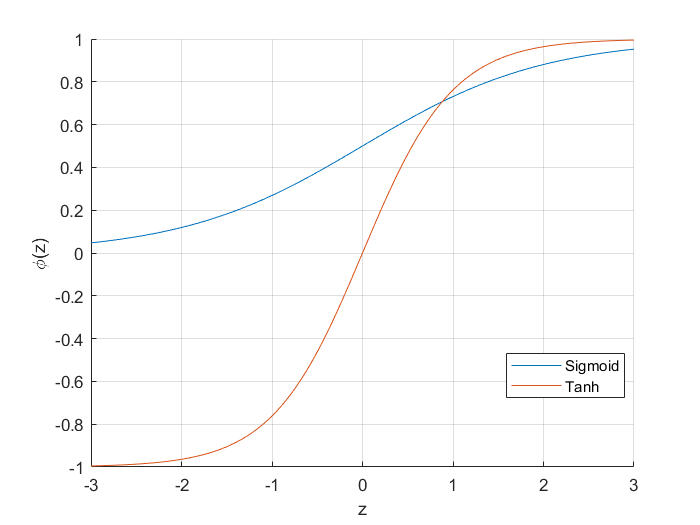
\includegraphics[width=0.4\linewidth]{sigVsTanh}
		\caption{Visualization of sigmoid and Tanh function}
		\label{fig:sigvstanh}
	\end{figure}

	Both functions have relativly simple mathematical formulas and are differentiable. In this paper the sigmoid function is used over the Tanh function, 
	
	The sigmoid function function is used over the Tanh function as it does not pass through the zero.  and 
	
	
	Sigmoid and Tanh are not the only activation functions. Other functions that should be noted are the Rectified Linear Unit (ReLU) and the Leaky Rectified Linear Unit function. While these functions can perform better than Tanh and Sigmoid, they are more complex and a proper discussion of them is outside the scope of this paper. 
	
	Expalain importance of activation function
	
	\subsection{Pitfalls}
	The most important thing to stear clear of is over traning. Overtraning occurs when the neural net trains too much to the traning data. While it will have a high accuracy for the traning data, it's performance for the test data will decay, as it has become too well attuned to the training data.  \par 
	
	The other problem is the time it takes to train. A three layer neural net can be trained to 97\% accuracy within 10 minutes, however it will not improve far beyond that. Larger nets will take longer to train, but will take far longer to train. 
	
	\begin{figure}
		\centering
		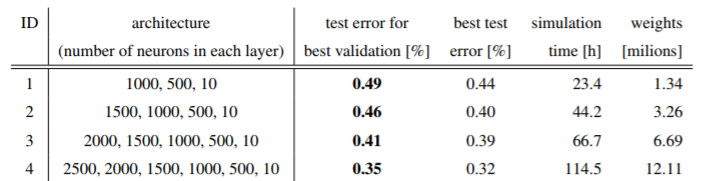
\includegraphics[width=0.7\linewidth]{nnRunTime}
		\caption{Run times for various neural network architectures\cite{deepBig}.}
		\label{fig:nnruntime}
	\end{figure}
	
	\section{Implementation}
	\subsection{Object Oriented Programming in MATLAB}
	This neural net had to be made without the use of any built in libraries \cite{Hicken18gradProjDes} and the code had to be modular \cite{Hicken18gradProjRubric}. TO create code for neural network subject to these constraints the author decided to create their own neural net class in MATLAB. \par 
	
	In MATLAB a class is an object that has parameters and functions. 
	
	The MATLAB class philipNeuralNet.m was written for this neural net project. It has the parameters learningRate and Level. The Level parameter has four parameters attached to it: W (weight), dW (weight derivative),  z (input), and A (the vector for the layer). By having this class we have avoided hard coding the propagation of the neural net and it is possible to test different neural net architectures on this code. 
	
	With these restrictions the 
	As this neural net 
	MATLAB allows 
	\subsection{MATLAB Code}
	NOTE THAT THIS CODE WAS BIAS FREE
	The code for this project was 
	The code written for this project was diuesgend so that the 
	
	For a three layer neural net a hidden layer of 250 neurons seems to work the best\cite{matlabNNBeg}. 
	
	Go over how it was implemented
	Go over batch testing
	
	restuls, comparison of diffrent arctiectures
	
	Go over the way this was implmented for the best way
	
	
	
	
	\section{Results}
	\subsection{Simple Neural Net}
	The best results were found for simplex neural net examined; a one hidden layer with 250 nodes a learning rate of 0.1, and no biases. 
	For a simple, $784\times250\times10$ neural net with a learning rate of 0.1 a test accuracy of 98\% was achieved. 
	
	
	
	Looking at the results,  It was discovered that
	
	\subsection{Comparison of different hidden layer sizes}
	
	\subsection{Multiple hidden layers}
	
	
	
	
	
	 %, Kepler, Newton, and Euler\cite{lectureOnGreekAstro}. 
	
	%\textcolor{red}{Segway hre}


	
	\section{Conclusion}
	
	The simple neural net achieved an accuracy of 98.37\%. This is on par with human recognition. 

			%--------------------------------------
		% References
		% -------------------------------------
		
		\bibliographystyle{unsrt}
		\bibliography{ref}

		
		%-----------------------------------------------------------
		% Appendix
		%-----------------------------------------------------------
		\newpage
		\singlespacing
%		\section*{Appendix 1 -derivation of gibbs}
		\section*{Appendix 1 - MATLAB code}
		\addcontentsline{toc}{section}{Appendix}
		
		\lstset{language=Matlab,%
			%basicstyle=\color{red},
			breaklines=true,%
			morekeywords={matlab2tikz},
			keywordstyle=\color{blue},%
			morekeywords=[2]{1}, keywordstyle=[2]{\color{black}},
			identifierstyle=\color{black},%
			stringstyle=\color{mylilas},
			commentstyle=\color{mygreen},%
			showstringspaces=false,%without this there will be a symbol in the places where there is a space
			numbers=left,%
			numberstyle={\tiny \color{black}},% size of the numbers
			numbersep=9pt, % this defines how far the numbers are from the text
			emph=[1]{for,end,break},emphstyle=[1]\color{red}, %some words to emphasise
			%emph=[2]{word1,word2}, emphstyle=[2]{style},    
		}
	\subsection*{NN\_Master.m}
	\lstinputlisting{C:/Users/Philip/Documents/GitHub/designOpNN/latexCode/NN_Master.m}
	\subsection*{philipNeuralNet.m}
	\lstinputlisting{C:/Users/Philip/Documents/GitHub/designOpNN/latexCode/philipNeuralNet.m}
	%\lstinputlisting{C:/Users/Philip/Documents/GitHub/Thesis/Master_TLE.m}
	%\lstinputlisting{C:/Users/Philip/Documents/GitHub/independent_study_fall_2018/Independat-Study-Fall-2018/Gibbs_Heck_master_loop_Latex.m}
	
	%\subsection{Code}
	%\subsection{Master\_TLE.m}
	%\lstinputlisting{C:/Users/Philip/Documents/GitHub/Thesis/Master_TLE.m}
	%\subsection{get\_SATCAT.m}
	%	\lstinputlisting{C:/Users/Philip/Documents/GitHub/Thesis/get_SATCAT.m}
	%	\subsection{get\_TLE\_from\_ID\_Manager.m}
	%\lstinputlisting{C:/Users/Philip/Documents/GitHub/Thesis/get_TLE_from_ID_Manager.m}
	
	%\subsection{get\_TLE\_from\_NorID.m}
	%\lstinputlisting{C:/Users/Philip/Documents/GitHub/Thesis/get_TLE_from_NorID.m}
	%\lstinputlisting{get_SATCAT.m}
	
	%Thanks for Paul McKee who started this template. It seems to have good matlab code viwing
		
	\end{document}
	
